\documentclass[12pt,letterpaper]{article}

\usepackage{arxiv}

\usepackage[utf8]{inputenc} % allow utf-8 input
\usepackage[T1]{fontenc}    % use 8-bit T1 fonts
\usepackage{hyperref}       % hyperlinks
\usepackage{url}            % simple URL typesetting
\usepackage{booktabs}       % professional-quality tables
\usepackage{amsfonts}       % blackboard math symbols
\usepackage{nicefrac}       % compact symbols for 1/2, etc.
\usepackage{microtype}      % microtypography
\usepackage{lipsum}
\usepackage{graphicx}	% Including figure files
\usepackage{mathtools}  %loads amsmath as well
\usepackage{amssymb}	% Extra maths symbols
\usepackage[english]{babel}
\usepackage{float}
\usepackage{bm}
\usepackage{indentfirst}
\usepackage{tikz}
\usetikzlibrary{positioning}
\usepackage{pgfplots}
\usepackage{color,soul}
%\pgfplotsset{compat=1.12}
\definecolor{mygray}{RGB}{125,125,125}
\definecolor{myred}{RGB}{255,60,60}
\definecolor{myblue}{RGB}{60,60,255}
\renewcommand{\arraystretch}{1.2}

% potential journals
% journal of computational physics
% computers and fluids
% international journal for numerical methods in fluids
% aiaa
% journal of fluid mechanics
\title{A Multiresolution Scheme Featuring Fully Adaptive Blocks for Simulating Reactive Flows}

\author{
  Brandon Gusto\\
  Department of Scientific Computing\\
  Florida State University\\
  Tallahassee, FL 32306 \\
  \texttt{bgusto@fsu.edu} \\
  %% examples of more authors
  \And
  Tomasz Plewa \\
  Department of Scientific Computing\\
  Florida State University\\
  Tallahassee, FL 32306 \\
  \texttt{tplewa@fsu.edu} \\
}

\begin{document}
\maketitle

\begin{abstract}
    We present a generalization of Harten's original multiresolution scheme for
    simulating reactive flows on logically rectangular block-structured adaptive
    mesh refinement (AMR) grids in one and two dimensions. The scheme addresses
    a major shortcoming of tree-based AMR codes, which is the creation of blocks
    with a low filling factor; that is, many cells in such a block are resolved
    beyond the desired error tolerance, necessitating excessive computational
    resources.  To overcome this issue, we introduce a multiresolution
    representation of the solution, not only to adapt the grid but also to
    adaptively compute fluxes and sources on each block. The scheme recycles
    regularity information obtained by the multiresolution grid adaptation in
    order to select flux and source calculations which may be accurately
    replaced by interpolation from the multiresolution basis. A block which
    employs this scheme is denoted as a fully adaptive block (FAB).  The error
    introduced by this approximation is shown to be of the same order as the
    local truncation error of the reconstruction scheme. Thus the rate of
    convergence of the underlying spatial reconstruction scheme is preserved.
    Additionally with respect to parallel applications, the multiresolution
    transform and computation of fluxes and sources on FABs is asynchronous,
    requiring only one synchronization step which is equivalent to the filling
    of ghost cells for each block. The efficiency of the scheme is demonstrated
    using several one and two-dimensional problems.
\end{abstract}

% keywords can be removed
\keywords{Multiresolution \and Adaptive Mesh Refinement \and Conservation Laws}

\section{Introduction}

    % paragraph introduces the need for spatially adaptive grids
    Fluid flows are often characterized by disparate spatial and temporal length
    scales. Certain features such as turbulence or shocks necessitate
    significantly higher resolution in computer simulations than smooth regions
    of the flow.  Naturally, intense effort has gone into the development of
    methods which employ a multi-scale or adaptive strategy to accurately
    simulate such flows without over-resolving smooth areas of the domain.

    % paragraph introducing adaptive mesh refinement as a concept
    The most popular strategy to accurately capture regions of interest in fluid
    simulations is to introduce a non-uniform spatial grid.  Methods which
    introduce a hierarchy of nested grid levels are generally described as
    adaptive mesh refinement (AMR) methods. Obtaining an estimate of the local
    truncation error (LTE) of the numerical scheme on a particular grid
    level allows for the identification of regions where refinement is necessary
    for solution accuracy. AMR methods may employ several strategies to
    approximate the LTE. 
    %\cite{Berger1984}.  Alternative methods include
    %feature-based refinement, and evaluation of gradient information (references
    %here).

    % paragraph reviews the work of harten and multiresolution methods
    An alternate approach to dynamic grid adaptation based on wavelets has became
    popular in recent years. The first such effort was introduced in a seminal
    paper by Harten \cite{harten1994}, where a multiresolution representation of
    the discrete solution on a uniform grid was used for adaptively computing the
    divergence of the flux within a finite volume formulation. The original
    scheme was applied soley to hyperbolic conservation laws, but was then
    expanded by Bihari to include viscous terms in (\hl{citation}), and then source
    terms in the context of reactive flows in (\hl{citation}). Harten's scheme
    represents the discrete solution on a uniform grid, but uses a
    multiresolution representation of the solution to identify regions where
    flux computations may be avoided. The multiresolution transform is obtained
    by using average-interpolating wavelets as basis functions. The scheme was
    extended to multiple dimensions in (cite), and the to problems with source
    terms in (cite).

    % review the multiresolution-adaptive papers
    Although Harten's original scheme was intended to be an alternative to
    spatially non-uniform grid adaptation, a series of papers have
    since reintroduced this concept within the MR framework. Thus the AMR
    approach has been redeveloped but with the refinement criterion defined by
    the MR representation rather than with the traditional metrics mentioned
    previously.

    % discuss pros cons of block-amr

\section{Governing Equations and Finite Volume Formulation}

    % describe merging block-structured AMR with Harten's scheme
    In the present work we are interested in numerically solving conservation
    laws of the form
    \begin{equation}
    \begin{cases}
      u_{t} + f(u)_{x} = s(u) \\    
      u(x,0) = u_{0}(x),
    \end{cases}
    \label{claw}
    \end{equation}
    where $u$ represents a conserved quantity, $f(u)$ is the flux function, and
    $s(u)$ is a source term. For the sake of presentation, we let the scalar
    equation (\ref{claw}) stand in for the more complicated systems of
    conversation laws which will be the focus of applications.  In the finite
    volume formulation, the solution $u(x,t)$ is approximated by volume
    averages defined within each cell $I_{i} = \left[ x_{i}-\frac{h}{2},
    x_{i}+\frac{h}{2} \right]$ in the computational domain.  The cell width $h$
    is determined by the number of cells, $N$, and the size of the domain
    $\Omega \in \left[a,b\right]$.
    The cell averages are given by
    \begin{equation}
        u_{i}(t) = \frac{1}{h} \int_{x_{i-1/2}}^{x_{i+1/2}} u(\xi,t) d \xi,
    \end{equation}
    where for convenience we use $i \pm 1/2$ in the subscripts to
    indicate the left and right interfaces of the target cell (i.e.
    $x_{i+1/2} =
    x_{i} + \frac{h}{2}$). The governing equations are cast into the
    semi-discrete conservative form,
    \begin{equation}
        \frac{du_{i}(t)}{dt} = -\frac{1}{h} \left( \hat{f}_{i+1/2} -
        \hat{f}_{i-1/2} \right),
    \end{equation}
    where the numerical flux is evaluated as
    \begin{equation}
        \hat{f}_{i + 1/2} = \hat{f}(u^{-}_{i+1/2}, u^{+}_{i+1/2}).
    \end{equation}
    In the present work, the reconstruction method of choice is a fifth-order
    weighted essentially non-oscillatory (WENO) scheme.

\section{Multiresolution Analysis}

    % overview of multiresolution
    In this section we first provide a brief review of the essential ideas
    regarding multiresolution analysis and wavelets as they pertain to the
    present work, and then we explain in-depth the muliresolution scheme used
    for both grid adaptation and the calculation of fluxes and sources.

    % describe multiresolution analysis (sourced from tymczak2000)
    A multiresolution analysis (MRA) of the Lebesgue space
    $L_{2}(\mathbb{R})$ defines a sequence of nested approximation spaces.
    These spaces satisfy certain self-similarity properties in both space
    and scale. An MRA defines the following sequence
    \begin{equation*}
        \dots \subset V_{j-1} \subset V_{j} \subset V_{j+1} \subset \dots \text{ }
        \text{ } \text{ } \text{ } j\in \mathbb{Z},
    \end{equation*}
    where for each subspace $V_{j}$,
    %, the points $y_{j}$ are defined. The
    %following properties hold:
    %\begin{enumerate}
    %    \item $f(x) \in V_{j} \Leftrightarrow f(x+k) \in V_{j} : \forall k
    %        \in y_{j}$
    %    \item $f(x) \in V_{j} \Leftrightarrow f(2x) \in V_{j+1}$ 
    %\end{enumerate}
    %The first point addresses the self-similarity in space, implying that
    %each subspace $V_{j}$ is invariant under shifts.
    a scaling function $\phi_{j}(x) \in V_{j}$ is defined which forms a basis,
    \begin{equation*}
        V_{j} = \text{span} \left\{ \phi_{j}(x+k) : \forall k \in y_{j}
        \right\}.
    \end{equation*}
    Additionally, the complement of $V_{j} \in V_{j+1}$ is $W_{j}$, which is
    known as the wavelet or detail space. This relation is defined
    by a direct summation as
    \begin{equation*}
        V_{j+1} = W_{j} \oplus V_{j}.
    \end{equation*}
    Considering successively finer approximation spaces yields
    \begin{equation*}
        V_j = V_0 \oplus W_0 \oplus W_1 \oplus \dots \oplus W_{j-1},
    \end{equation*}
    thus fine-scale information on any arbitrary level $j$ is represented by
    the coarsest scale plus a series of differences at higher levels.

\section{Harten's Multiresolution Scheme on Uniform Grids}

    % describe overview of transform, and average-interpolating wavelets
    The multiresolution scheme presented here is based on the work of Harten, as
    mentioned previously. The multiresolution analysis generated by this scheme
    consists of generalized bi-orthogonal wavelets (\hl{cite}). Although the
    wavelets are never constructed explicitly, the same mechanics used to build
    them are used to construct the multiresolution representation of the
    discrete solution.  This is done using average-interpolating polynomials to
    predict, based on a stencil of cell-averages at one grid level, the cell
    averages at one finer level of resolution. This process is done in a
    principled way, and defines the forward wavelet transform (also known as
    encoding). The transform consists of two steps:
    \begin{enumerate}
        \item[] \textbf{Split}: The cells at grid level $l$ are split into even and odd
                components.
        \item[] \textbf{Predict}: The odd cell averages at level $l$ are predicted
                by an average-interpolating polynomial based on cells at
                level $l-1$.
    \end{enumerate}
    Once the prediction step is complete, the difference information is
    easily obtained by comparing the odd-indexed cell-averages at level $l$ with
    their prediced values. The scheme is detailed by first examining the grid
    hierarchy needed for the multiresolution representation of the data.

    \subsection*{Grid Hierarchy}

        % describe the nested grids
        In Harten's original scheme, the domain is discretized into a
        hierarchy of uniformly-spaced, nested grids. In Cartesian
        coordinates, the grid is defined by
        \begin{equation}
            \mathcal{G}^{l} = \left\{ x_{i}^{l} \right\}_{i=0}^{N^{l}}, \text{ }
            \text{ } \text{ } \text{ } x_{i}^{l} = i \cdot h^{l}, \text{ }
            \text{ } h^{l} = 2^{l} \cdot h^{0}, \text{ } \text{ } N^{l} = N_{0}
            / 2^{l},
        \end{equation}
        where on level $l$, $h^{l}$ is the cell width and $N^{l}$ is the number of cells.

        % illustration of grids here?

    \subsection*{Forward Transform}

        % describe the prediction operator, and detail coefficients
        The forward transform provides regularity information about the function
        underlying the fine-grid data. The transform procedure can be succinctly
        written in terms of a matrix-vector operation to yield the
        multiresolution representation of the data, $u_{MR}^{0}$, as
        \begin{equation}
            \bm{u}_{M}^{l} = \bm{M}^{l} \bm{u}^{l} = \left( \bm{d}^{l+1}, \bm{d}^{l+2},
            \dots, \bm{d}^{l+L}; \bm{u}^{L} \right)^{T}.
        \end{equation}
        Here the multiresolution operator $\bm{M}$ contains the prediction
        operator for each
        \begin{equation}
            \tilde{u}_{2i+1}^{l-1} \approx u_{i}^{l} - \sum_{p=1}^{s}
            \gamma_{p} \left( u^{l}_{i-p} - u^{l}_{i+p} \right).
        \end{equation}
        In Table (1) the coefficients are shown for several average-interpolating stencils
        \begin{table}
            \centering
            \begin{tabular}{|l|l|l|l|}
            \hline
                & $\gamma_{1}$ & $\gamma_{2}$ & $\gamma_{3}$ \\ \hline
                $s=1$ & $1/8$ & 0 & 0 \\ \hline
                $s=2$ & $-22/128$ & $3/128$ & 0 \\ \hline
            \end{tabular}
            \caption{Coefficients for cell-average interpolation in the prediction step.}
        \end{table}
        The detail coefficients are then computed as
        \begin{equation}
            d^{l}_{i} = u^{l-1}_{2i+1} - \tilde{u}^{l-1}_{2i+1}.
        \end{equation}
        These steps are illustrated in Figure (2).

        % illustration of parallel fwt 
        \begin{figure}[H]
            \center
            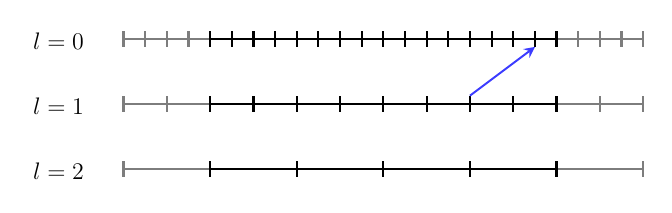
\begin{tikzpicture}[thick,scale=0.275, every node/.style={scale=0.6}]

    % variables
    \def\xl{-8.0}
    \def\xr{8.0}
    \def\y{0.0}
    \def\yy{-3.0}
    \def\yyy{-6.0}
    \def\ts{0.75}
    \def\op{0.35}
    \def\fx{0.15}
    
    % draw ghost cells
    \draw [mygray] (\xl-4,\y+\ts/2) --(\xr+4,\y+\ts/2);
    \draw [mygray] (\xl-4,\yy+\ts/2) --(\xr+4,\yy+\ts/2);
    \draw [mygray] (\xl-4,\yyy+\ts/2) --(\xr+4,\yyy+\ts/2);
    \draw [mygray] (\xl-1.0,\y) --(\xl-1.0,\y+\ts);
    \draw [mygray] (\xr+1.0,\y) --(\xr+1.0,\y+\ts);
    \draw [mygray] (\xl-2.0,\y) --(\xl-2.0,\y+\ts);
    \draw [mygray] (\xr+2.0,\y) --(\xr+2.0,\y+\ts);
    \draw [mygray] (\xl-3.0,\y) --(\xl-3.0,\y+\ts);
    \draw [mygray] (\xr+3.0,\y) --(\xr+3.0,\y+\ts);
    \draw [mygray] (\xl-4.0,\y) --(\xl-4.0,\y+\ts);
    \draw [mygray] (\xr+4.0,\y) --(\xr+4.0,\y+\ts);

    % ghost cells at level l=1
    \draw [mygray] (\xl-2.0,\yy) --(\xl-2.0,\yy+\ts);
    \draw [mygray] (\xr+2.0,\yy) --(\xr+2.0,\yy+\ts);
    \draw [mygray] (\xl-4.0,\yy) --(\xl-4.0,\yy+\ts);
    \draw [mygray] (\xr+4.0,\yy) --(\xr+4.0,\yy+\ts);

    % level l=2
    \draw [mygray] (\xl-4.0,\yyy) --(\xl-4.0,\yyy+\ts);
    \draw [mygray] (\xr+4.0,\yyy) --(\xr+4.0,\yyy+\ts);

    % draw grids
    \draw (\xl,\y+\ts/2) --(\xr,\y+\ts/2);
    \draw (\xl,\yy+\ts/2) --(\xr,\yy+\ts/2);
    \draw (\xl,\yyy+\ts/2) --(\xr,\yyy+\ts/2);
    
    % draw cells for max level
    \draw (\xl,\y) --(\xl,\y+\ts);
    \draw (\xl+1.0,\y) --(\xl+1.0,\y+\ts);
    \draw (\xl+2.0,\y) --(\xl+2.0,\y+\ts);
    \draw (\xl+3.0,\y) --(\xl+3.0,\y+\ts);
    \draw (\xl+4.0,\y) --(\xl+4.0,\y+\ts);
    \draw (\xl+5.0,\y) --(\xl+5.0,\y+\ts);
    \draw (\xl+6.0,\y) --(\xl+6.0,\y+\ts);
    \draw (\xl+7.0,\y) --(\xl+7.0,\y+\ts);
    \draw (\xl+8.0,\y) --(\xl+8.0,\y+\ts);
    \draw (\xl+9.0,\y) --(\xl+9.0,\y+\ts);
    \draw (\xl+10.0,\y) --(\xl+10.0,\y+\ts);
    \draw (\xl+11.0,\y) --(\xl+11.0,\y+\ts);
    \draw (\xl+12.0,\y) --(\xl+12.0,\y+\ts);
    \draw (\xl+13.0,\y) --(\xl+13.0,\y+\ts);
    \draw (\xl+14.0,\y) --(\xl+14.0,\y+\ts);
    \draw (\xl+15.0,\y) --(\xl+15.0,\y+\ts);
    \draw (\xl+16.0,\y) --(\xl+16.0,\y+\ts);
    
    % lower level cells
    \draw (\xl,\yy) --(\xl,\yy+\ts);
    \draw (\xl+2.0,\yy) --(\xl+2.0,\yy+\ts);
    \draw (\xl+4.0,\yy) --(\xl+4.0,\yy+\ts);
    \draw (\xl+6.0,\yy) --(\xl+6.0,\yy+\ts);
    \draw (\xl+8.0,\yy) --(\xl+8.0,\yy+\ts);
    \draw (\xl+10.0,\yy) --(\xl+10.0,\yy+\ts);
    \draw (\xl+12.0,\yy) --(\xl+12.0,\yy+\ts);
    \draw (\xl+14.0,\yy) --(\xl+14.0,\yy+\ts);
    \draw (\xl+16.0,\yy) --(\xl+16.0,\yy+\ts);
    
    % even lower level cells
    \draw (\xl,\yyy) --(\xl,\yyy+\ts);
    \draw (\xl+4.0,\yyy) --(\xl+4.0,\yyy+\ts);
    \draw (\xl+8.0,\yyy) --(\xl+8.0,\yyy+\ts);
    \draw (\xl+12.0,\yyy) --(\xl+12.0,\yyy+\ts);
    \draw (\xl+16.0,\yyy) --(\xl+16.0,\yyy+\ts);
 
    % arrows indicating flux interpolation dependency
    \draw[myblue,->,line width=0.25mm,>=stealth] (\xr-4,\yy+\ts) -- (\xr-1,\y);

    % nodes
    \node at (\xl-7.0,\y+0.25) {\Large $l=0$};
    \node at (\xl-7.0,\yy+0.25) {\Large $l=1$};
    \node at (\xl-7.0,\yyy+0.25) {\Large $l=2$};

\end{tikzpicture}

            \caption{A block of consisting of $N^{0} = 16$ cells is shown. Four
            ghost cells are included on each end of the block, allowing the
            multiresolution decomposition to descend two levels (to grid level
            $l=2$). Interpolation stencils for the computation of detail
            coefficients at levels $l=1, l=2$ are shown, indicating the need for ghost cells.}
        \end{figure}

    \subsection*{Inverse Transform}

        % 
        
    \subsection*{Calculation of Fluxes and Sources}
        Once the detail coefficients have been obtained, the MR scheme
        proceeds by setting a threshold $\epsilon$ and truncating coefficients
        which have an absolute value below the threshold. Lastly, the inverse
        transform then starts from grid $l=L$ and at each interface either
        computes fluxes using the fine-grid scheme, or interpolates them using
        the MR basis. The fluxes are interpolated by
        \begin{align}
            & \tilde{f}_{2i+1}^{l-1} \approx \sum_{p=1}^{s+1} \alpha_{p} \left(
            \hat{f}^{l}_{i-p+1} + \hat{f}^{l}_{i+p} \right),
        \end{align}
        where the interpolants are of degree $2s+1$. The coefficients for
        various degrees of polynomial interpolants are shown in Table (ref).
        \begin{table}
            \centering
            \begin{tabular}{|l|l|l|l|}
            \hline
                & $\alpha_{1}$ & $\alpha_{2}$ & $\alpha_{3}$ \\ \hline
                $s=0$ & 1/2 & 0 & 0 \\ \hline
                $s=1$ & 9/16 & -1/16 & 0 \\ \hline
            \end{tabular}
            \caption{Coefficients for cell-average interpolation in the prediction step.}
        \end{table}
        The process repeats until all fluxes are either computed or
        interpolated on the fine grid $l=0$.

        \subsection*{Error Analysis}

            % describe choice of epsilon

\section{Asynchronous Fully Adaptive Block Scheme}

    % two main issues: no jump greater than one refinement level, and no
    % incomplete trees

    % illustration amr block tree structure
    \begin{figure}[H]
        \center
        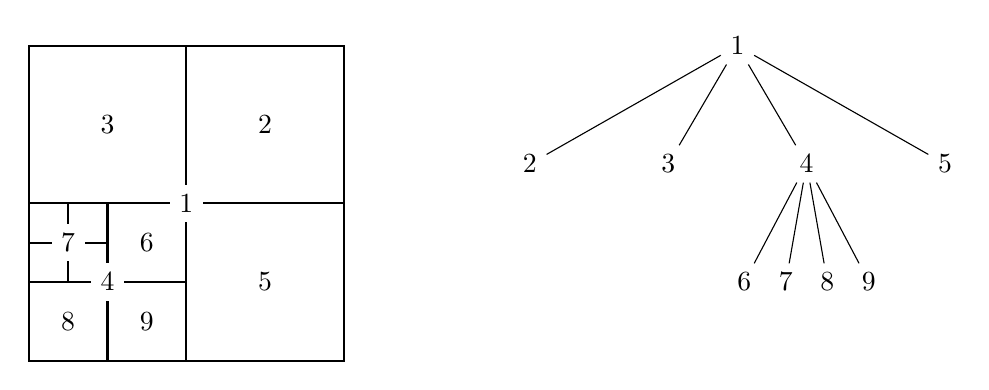
\begin{tikzpicture}[sibling distance=5em,every node/.style = {shape=rectangle,align=center,top color=white}]

    % draw amr blocks
    \draw [thick] (0,0) rectangle (4,4);
    \draw [thick] (2,2) rectangle (4,4);
    \draw [thick] (0,0) rectangle (2,2);
    \draw [thick] (0,0) rectangle (1,1);
    \draw [thick] (1,1) rectangle (2,2);
    \draw [thick] (0,1) rectangle (0.5,1.5);
    \draw [thick] (0.5,1.5) rectangle (1,2);

    % block labels
    \node [shape=rectangle,align=center] at (2,2) {1};
    \node [shape=rectangle,align=center] at (3,3) {2};
    \node [shape=rectangle,align=center] at (1,3) {3};
    \node [shape=rectangle,align=center] at (1,1) {4};
    \node [shape=rectangle,align=center] at (3,1) {5};
    \node [shape=rectangle,align=center] at (1.5,1.5) {6};
    \node [shape=rectangle,align=center] at (0.5,1.5) {7};
    \node [shape=rectangle,align=center] at (0.5,0.5) {8};
    \node [shape=rectangle,align=center] at (1.5,0.5) {9};

    \node at (9,4) {1}
        child { node {2} }
        child { node {3} }
        child { node {4}[sibling distance=1.5em,every node/.style = {shape=rectangle,align=center,top color=white}]
            child { node {6} }
            child { node {7} }
            child { node {8} }
            child { node {9} } }
        child { node {5} };

\end{tikzpicture}

        \caption{}
    \end{figure}

    % pseudocode of algorithm

    % illustration of parallel issue
    \begin{figure}[H]
        \center
        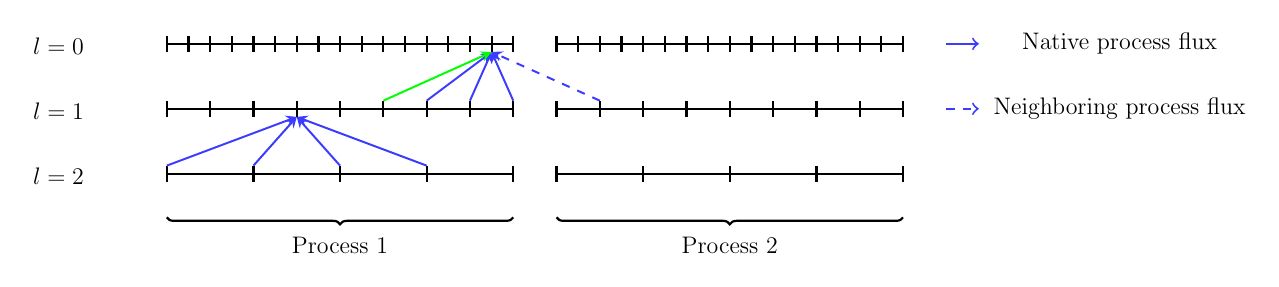
\begin{tikzpicture}[thick,scale=0.275, every node/.style={scale=0.6}]

    % variables
    \def\xl{-8.0}
    \def\xr{8.0}
    \def\y{0.0}
    \def\yy{-3.0}
    \def\yyy{-6.0}
    \def\ts{0.75}
    \def\op{0.35}
    \def\fx{0.15}
    
    % draw grids
    \draw (\xl,\y+\ts/2) --(\xr,\y+\ts/2);
    \draw (\xl,\yy+\ts/2) --(\xr,\yy+\ts/2);
    \draw (\xl,\yyy+\ts/2) --(\xr,\yyy+\ts/2);
    
    % draw cells for max level
    \draw (\xl,\y) --(\xl,\y+\ts);
    \draw (\xl+1.0,\y) --(\xl+1.0,\y+\ts);
    \draw (\xl+2.0,\y) --(\xl+2.0,\y+\ts);
    \draw (\xl+3.0,\y) --(\xl+3.0,\y+\ts);
    \draw (\xl+4.0,\y) --(\xl+4.0,\y+\ts);
    \draw (\xl+5.0,\y) --(\xl+5.0,\y+\ts);
    \draw (\xl+6.0,\y) --(\xl+6.0,\y+\ts);
    \draw (\xl+7.0,\y) --(\xl+7.0,\y+\ts);
    \draw (\xl+8.0,\y) --(\xl+8.0,\y+\ts);
    \draw (\xl+9.0,\y) --(\xl+9.0,\y+\ts);
    \draw (\xl+10.0,\y) --(\xl+10.0,\y+\ts);
    \draw (\xl+11.0,\y) --(\xl+11.0,\y+\ts);
    \draw (\xl+12.0,\y) --(\xl+12.0,\y+\ts);
    \draw (\xl+13.0,\y) --(\xl+13.0,\y+\ts);
    \draw (\xl+14.0,\y) --(\xl+14.0,\y+\ts);
    \draw (\xl+15.0,\y) --(\xl+15.0,\y+\ts);
    \draw (\xl+16.0,\y) --(\xl+16.0,\y+\ts);
    
    % lower level cells
    \draw (\xl,\yy) --(\xl,\yy+\ts);
    \draw (\xl+2.0,\yy) --(\xl+2.0,\yy+\ts);
    \draw (\xl+4.0,\yy) --(\xl+4.0,\yy+\ts);
    \draw (\xl+6.0,\yy) --(\xl+6.0,\yy+\ts);
    \draw (\xl+8.0,\yy) --(\xl+8.0,\yy+\ts);
    \draw (\xl+10.0,\yy) --(\xl+10.0,\yy+\ts);
    \draw (\xl+12.0,\yy) --(\xl+12.0,\yy+\ts);
    \draw (\xl+14.0,\yy) --(\xl+14.0,\yy+\ts);
    \draw (\xl+16.0,\yy) --(\xl+16.0,\yy+\ts);
    
    % even lower level cells
    \draw (\xl,\yyy) --(\xl,\yyy+\ts);
    \draw (\xl+4.0,\yyy) --(\xl+4.0,\yyy+\ts);
    \draw (\xl+8.0,\yyy) --(\xl+8.0,\yyy+\ts);
    \draw (\xl+12.0,\yyy) --(\xl+12.0,\yyy+\ts);
    \draw (\xl+16.0,\yyy) --(\xl+16.0,\yyy+\ts);
    
    % curly brace
    \draw[decoration={brace,mirror,raise=5pt},decorate]
        (\xl,\yyy-1.0) -- node[below=10pt] {\Large Process 1}(\xr,\yyy-1.0);

    % arrows indicating flux interpolation dependency
    \draw[myblue,->,line width=0.25mm,>=stealth] (\xr-4,\yy+\ts) -- (\xr-1,\y);
    \draw[myblue,->,line width=0.25mm,>=stealth] (\xr-2,\yy+\ts) -- (\xr-1,\y);
    \draw[myblue,->,line width=0.25mm,>=stealth] (\xr,\yy+\ts) -- (\xr-1,\y);
    \draw[myblue,dashed,->,line width=0.25mm,>=stealth] (\xr+4,\yy+\ts) -- (\xr-1,\y);
    \draw[green,->,line width=0.25mm,>=stealth] (\xr-6,\yy+\ts) -- (\xr-1,\y);

    \draw[myblue,->,line width=0.25mm,>=stealth] (\xr-16,\yyy+\ts) -- (\xr-10,\yy);
    \draw[myblue,->,line width=0.25mm,>=stealth] (\xr-12,\yyy+\ts) -- (\xr-10,\yy);
    \draw[myblue,->,line width=0.25mm,>=stealth] (\xr-8,\yyy+\ts) -- (\xr-10,\yy);
    \draw[myblue,->,line width=0.25mm,>=stealth] (\xr-4,\yyy+\ts) --(\xr-10,\yy);

    % nodes
    \node at (\xl-5.0,\y+0.25) {\Large $l=0$};
    \node at (\xl-5.0,\yy+0.25) {\Large $l=1$};
    \node at (\xl-5.0,\yyy+0.25) {\Large $l=2$};

    % draw process 2 grid
    \def\xl{10.0}
    \def\xr{26.0}
    \draw (\xl,\y+\ts/2) --(\xr,\y+\ts/2);
    \draw (\xl,\yy+\ts/2) --(\xr,\yy+\ts/2);
    \draw (\xl,\yyy+\ts/2) --(\xr,\yyy+\ts/2);
    
    % draw cells for max level
    \draw (\xl,\y) --(\xl,\y+\ts);
    \draw (\xl+1.0,\y) --(\xl+1.0,\y+\ts);
    \draw (\xl+2.0,\y) --(\xl+2.0,\y+\ts);
    \draw (\xl+3.0,\y) --(\xl+3.0,\y+\ts);
    \draw (\xl+4.0,\y) --(\xl+4.0,\y+\ts);
    \draw (\xl+5.0,\y) --(\xl+5.0,\y+\ts);
    \draw (\xl+6.0,\y) --(\xl+6.0,\y+\ts);
    \draw (\xl+7.0,\y) --(\xl+7.0,\y+\ts);
    \draw (\xl+8.0,\y) --(\xl+8.0,\y+\ts);
    \draw (\xl+9.0,\y) --(\xl+9.0,\y+\ts);
    \draw (\xl+10.0,\y) --(\xl+10.0,\y+\ts);
    \draw (\xl+11.0,\y) --(\xl+11.0,\y+\ts);
    \draw (\xl+12.0,\y) --(\xl+12.0,\y+\ts);
    \draw (\xl+13.0,\y) --(\xl+13.0,\y+\ts);
    \draw (\xl+14.0,\y) --(\xl+14.0,\y+\ts);
    \draw (\xl+15.0,\y) --(\xl+15.0,\y+\ts);
    \draw (\xl+16.0,\y) --(\xl+16.0,\y+\ts);
    
    % lower level cells
    \draw (\xl,\yy) --(\xl,\yy+\ts);
    \draw (\xl+2.0,\yy) --(\xl+2.0,\yy+\ts);
    \draw (\xl+4.0,\yy) --(\xl+4.0,\yy+\ts);
    \draw (\xl+6.0,\yy) --(\xl+6.0,\yy+\ts);
    \draw (\xl+8.0,\yy) --(\xl+8.0,\yy+\ts);
    \draw (\xl+10.0,\yy) --(\xl+10.0,\yy+\ts);
    \draw (\xl+12.0,\yy) --(\xl+12.0,\yy+\ts);
    \draw (\xl+14.0,\yy) --(\xl+14.0,\yy+\ts);
    \draw (\xl+16.0,\yy) --(\xl+16.0,\yy+\ts);
    
    % even lower level cells
    \draw (\xl,\yyy) --(\xl,\yyy+\ts);
    \draw (\xl+4.0,\yyy) --(\xl+4.0,\yyy+\ts);
    \draw (\xl+8.0,\yyy) --(\xl+8.0,\yyy+\ts);
    \draw (\xl+12.0,\yyy) --(\xl+12.0,\yyy+\ts);
    \draw (\xl+16.0,\yyy) --(\xl+16.0,\yyy+\ts);
    
    % curly brace
    \draw[decoration={brace,mirror,raise=5pt},decorate]
        (\xl,\yyy-1.0) -- node[below=10pt] {\Large Process 2}(\xr,\yyy-1.0);

    % legend
    \draw[myblue,->,line width=0.25mm] (\xr+2,\y+\ts/2) -- (\xr+3.5,\y+\ts/2);
    \draw[myblue,->,dashed,line width=0.25mm] (\xr+2,\yy+\ts/2) -- (\xr+3.5,\yy+\ts/2);
    \node at (\xr+10,\y+\ts/2) {\Large Native process flux};
    \node at (\xr+10,\yy+\ts/2) {\Large Neighboring process flux};

\end{tikzpicture}

       \caption{Two examples of flux interpolation on a hierarchy of grids
        on Process 1: one procedure requires flux data from the adjacent
        process, the other does not.}
    \end{figure}

    \subsection*{Buffer Region}

    \subsection*{Load Balancing}

\section{Numerical Results}

    \subsection*{Convergence Analysis}

        \begin{center}\vspace{1cm}
        \begin{tabular}{|l|l|l|l|l|l|l|l|l|}
        \hline
                   & \multicolumn{4}{l|}{$\epsilon = 0.0$}              & \multicolumn{4}{l|}{$\epsilon = 10^{-12}$}         \\ \hline
        grid cells & $L_{1}$ error & order & $L_{\infty}$ error & order & $L_{1}$ error & order & $L_{\infty}$ error & order \\ \hline
        16         &               &       &                    &       &               &       &                    &       \\ \hline
        32         &               &       &                    &       &               &       &                    &       \\ \hline
        64         &               &       &                    &       &               &       &                    &       \\ \hline
        128        &               &       &                    &       &               &       &                    &       \\ \hline
        256        &               &       &                    &       &               &       &                    &       \\ \hline
                   & \multicolumn{4}{l|}{$\epsilon = 10^{-6}$}          & \multicolumn{4}{l|}{$\epsilon = 10^{-4}$}          \\ \hline
        grid cells & $L_{1}$ error & order & $L_{\infty}$ error & order & $L_{1}$ error & order & $L_{\infty}$ error & order \\ \hline
        16         &               &       &                    &       &               &       &                    &       \\ \hline
        32         &               &       &                    &       &               &       &                    &       \\ \hline
        64         &               &       &                    &       &               &       &                    &       \\ \hline
        128        &               &       &                    &       &               &       &                    &       \\ \hline
        256        &               &       &                    &       &               &       &                    &       \\ \hline
        \end{tabular}
        \end{center}\vspace{1cm}

    \subsection*{Example}
    Using the inviscid flow assumption, the dynamics of compressible fluids are
    modeled using the reactive Euler equations \hl{add domain notation}
    \begin{equation}
       u_{t} + f(u)_{x}
       + g(u)_{y} = s(u),
        \label{goveq}
    \end{equation}
    where $u = \left( \rho, \rho u, \rho v, \rho w, E \right)^{T}$ is
    the state vector, the flux vectors are given by
    \begin{equation}
        f = 
    \begin{pmatrix}
    \rho u \\ \rho u^2 + p \\ \rho u v \\ \rho u w \\ u( E + p )
    \end{pmatrix}, \text{ } \text{ } \text{ }
        g = 
    \begin{pmatrix}
    \rho v \\ \rho u v \\ \rho v^2 + p \\ \rho v w \\ v( E + p )
    \end{pmatrix}, \text{ } \text{ } \text{ }
        h = 
    \begin{pmatrix}
    \rho w \\ \rho u w \\ \rho v w \\ \rho w^2 + p \\ w( E + p )
    \end{pmatrix},
    \end{equation}
    and $s(u)$ represents sources. The total energy per
    unit volume is given by
    \begin{equation*}
        E = \rho \left( \frac{1}{2} \mathbf{V}^{2} + e \right),
    \end{equation*}
    where $e$ is the internal energy and the kinetic energy contribution is
    \begin{equation*}
        \frac{1}{2} \mathbf{V}^{2} = \frac{1}{2} \mathbf{V}
        \cdot \mathbf{V} = \frac{1}{2} \left( u^2 + v^2 + w^2 \right).
    \end{equation*}
    The system of nonlinear equations is closed by an
    equation of state which is in general not derived from that of an ideal gas.

\section{Acknowledgements}

\appendix

\section{Derivation of Prediction Operator in One-Dimension}
We are interested in obtaining the difference between approximation spaces at varying levels of resolution. We 
are given cell-averaged values as input data to our wavelet transform. This data is fed to the scheme at some arbitrary maximum
resolution level $J$, and the wavelet transform produces details coefficients at each lower level until the coarsest level,
$j=0$, is reached. The coefficients in this case are interchangeable with the cell-averages and are denoted by $c^{j}_{k}$,
where the level of resolution is denoted by $j$, and the spatial index is denoted by $k$. We consider an interpolating
polynomial $p(x)$ such that 
\begin{align}
    c^{j}_{k-1} &= \int_{x^{j}_{k-1}}^{x^{j}_{k}} p(x) dx \\
    c^{j}_{k} &= \int_{x^{j}_{k}}^{x^{j}_{k+1}} p(x) dx \\
    c^{j}_{k+1} &= \int_{x^{j}_{k+1}}^{x^{j}_{k+2}} p(x) dx.
\end{align}
The polynomial $p(x)$ should then predict the finer cell-averages of cell $c^{j}_{k}$ as
\begin{align}
    \hat{c}^{j+1}_{2k} &= 2 \int_{x^{j}_{k}}^{x^{j}_{k+1/2}} p(x) dx \\
    \hat{c}^{j+1}_{2k+1} &= 2 \int_{x^{j}_{k+1/2}}^{x^{j}_{k+1}} p(x) dx
\end{align}
At present, it may not be clear how to implement such a scheme on a computer. However this interpolation procedure
can be cast in a more suitable form by introducing another polynomial, the integral of $p(x)$:
\begin{equation}
	P(x) = \int_{0}^{x} p(y) dy.
\end{equation}
Now the problem is to interpolate the following data
\begin{align}
    0 &= P(x^{j}_{k-1}) \\
    c^{j}_{k-1} &= P(x^{j}_{k}) \\
    c^{j}_{k-1} + c^{j}_{k} &= P(x^{j}_{k+1}) \\
    c^{j}_{k-1} + c^{j}_{k} + c^{j}_{k+1} &= P(x^{j}_{k+2}).
\end{align}
This can easily be done using Lagrange polynomials. Then the predictions are given in terms of $P(x)$ by
\begin{align}
	\hat{c}^{j+1}_{2k} &= 2 \left( P(x^{j}_{k+1/2}) - P(x^{j}_{k}) \right) \\
	\hat{c}^{j+1}_{2k+1} &= 2 \left( P(x^{j}_{k+1}) - P(x^{j}_{k+1/2}) \right).
\end{align}
This interpolating polynomial is cast in the Lagrange form,
\begin{equation}
P(x) = \sum_{i=0}^{n} y_{i} l_{i}(x),
\end{equation}
where $y_{i}$ are the functional data, and $l_{i}(x)$ are the Lagrange polynomials. For $n=3$ these
are given by
\begin{align}
    l_{0}(x) &= \frac{x-x_1}{x_0-x_1} \frac{x-x_2}{x_0-x_2} \frac{x-x_3}{x_0-x_3} \\
    l_{1}(x) &= \frac{x-x_0}{x_1-x_0} \frac{x-x_2}{x_1-x_2} \frac{x-x_3}{x_1-x_3} \\
    l_{2}(x) &= \frac{x-x_0}{x_2-x_0} \frac{x-x_1}{x_2-x_1} \frac{x-x_3}{x_2-x_3} \\
    l_{3}(x) &= \frac{x-x_0}{x_3-x_0} \frac{x-x_1}{x_3-x_1} \frac{x-x_2}{x_3-x_2},
\end{align}
and the final interpolating polynomial is
\begin{equation}
	P(x) = (0) l_{0}(x) + ( c^{j}_{k-1} ) l_{1}(x) + ( c^{j}_{k-1} + c^{j}_{k} ) l_{2}(x)
		+ ( c^{j}_{k-1} + c^{j}_{k} + c^{j}_{k+1} ) l_{3}(x).
\end{equation}
Several evaluations are necessary in order to obtain the predictions. Using intervals of equal length, these values are
\begin{align}
	P(x^{j}_{k}) &= c^{j}_{k-1} \\
	P(x^{j}_{k+1/2}) &= \frac{17}{16} c^{j}_{k-1} + \frac{1}{2} c^{j}_{k} - \frac{1}{16} c^{j}_{k+1} \\
	P(x^{j}_{k+1}) &= c^{j}_{k-1} + c^{j}_{k}.
\end{align}
Then the predictions of the cell-averages at the higher level of resolution are finally given by
\begin{align}
	\hat{c}^{j+1}_{2k} & = c^{j}_{k} + \frac{1}{8} \left( c^{j}_{k-1} - c^{j}_{k+1} \right) \\
	\hat{c}^{j+1}_{2k+1} & = c^{j}_{k} - \frac{1}{8} \left( c^{j}_{k-1} - c^{j}_{k+1} \right).
\end{align}
This procedure could easily be extended to non-uniformly
spaced intervals, giving different weights. Note that only the
odd indices are counted because in the multiresolution scheme the
data is initially split into even
and odd signals. All data at level $j$ are just considered to
be a copy of the even-index data at level $j+1$, whereas
the odd-indexed data at level $j+1$ is what is predicted
by even-indexed data at level $j+1$. Also important are the
interpolants at the ends of the domain. Given below are the
left and right predictions, respectively:
\begin{align}
	\hat{c}^{j+1}_{2k+1} & = \frac{5}{8} c^{j}_{k}
	+ \frac{1}{2} c^{j}_{k+1} - \frac{1}{8} c^{j}_{k+2} \\
	\hat{c}^{j+1}_{2k+1} & = \frac{1}{8} c^{j}_{k-2}
	- \frac{1}{2} c^{j}_{k-1} + \frac{11}{8} c^{j}_{k}.
\end{align}

\bibliographystyle{unsrt}  
\bibliography{references}

\end{document}
